\begin{figure}[ht!]
\centering
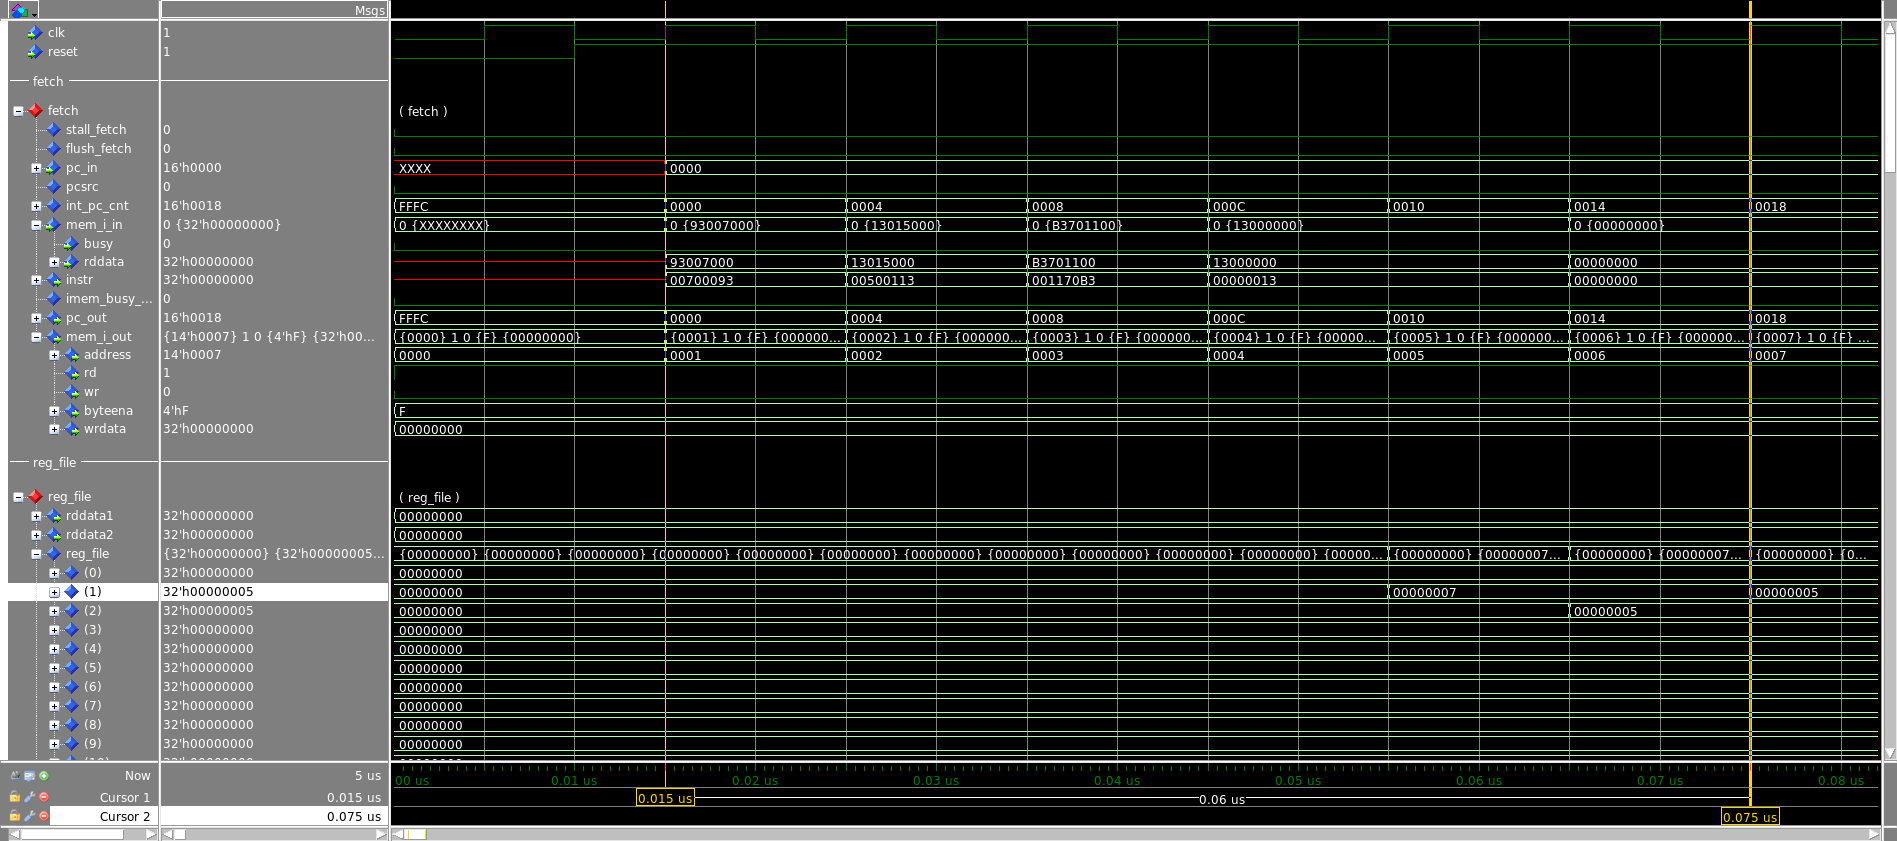
\includegraphics[width=1.0\linewidth]{task_1_fetch_regfile.png}
\caption{Simulation screenshot for Listing~\ref{lst:asmfwd_1}.}
\label{fig:sim1}
\end{figure}

\begin{figure}[ht!]
\centering
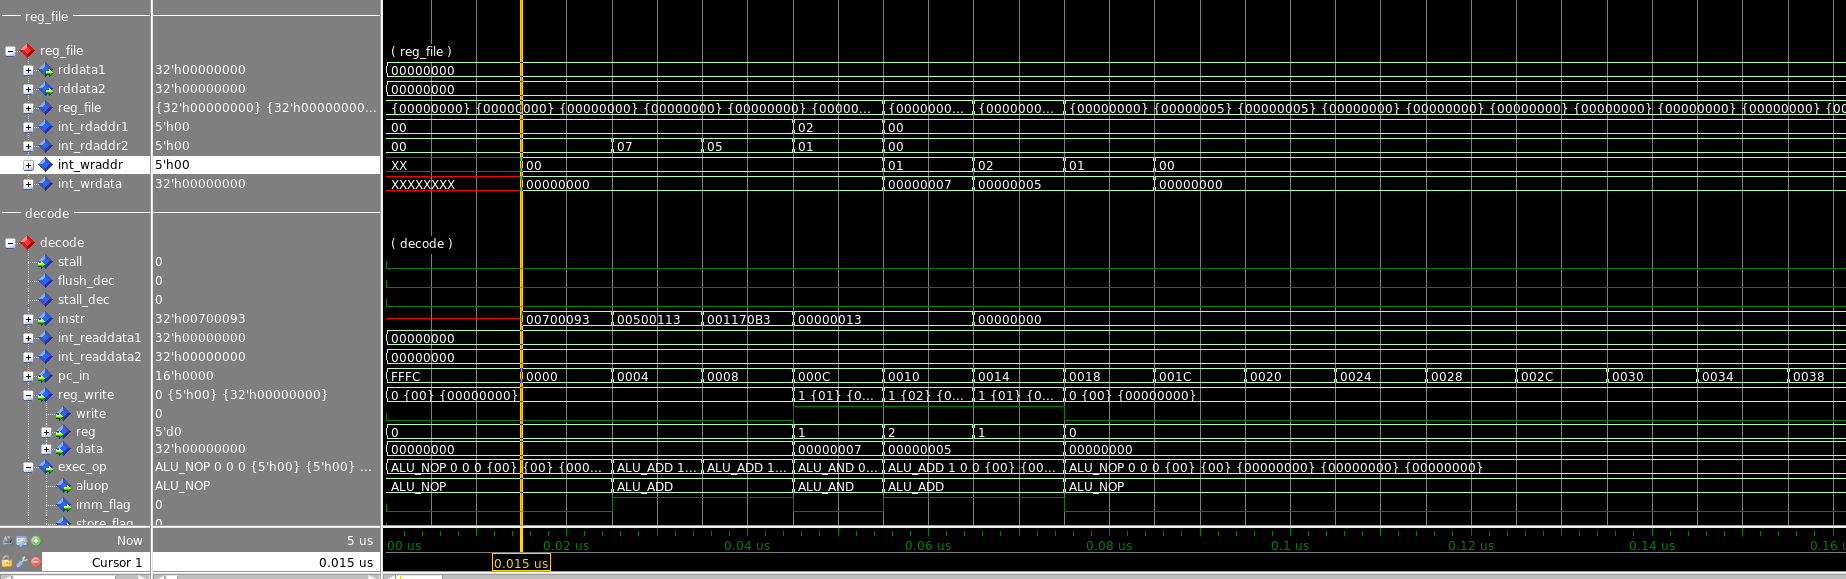
\includegraphics[width=1.0\linewidth]{task_1_regwrite.png}
\caption{The internal signal wraddr and wrdata.}
\label{fig:sim2}
\end{figure}
Unfortunately the signal \texttt{regwrite} was optimized away by the compiler. But you can see the
signal that causes the regfile to write values in the decode stage. There it is the signal \texttt{reg\_write.write}.

\begin{figure}[ht!]
\centering
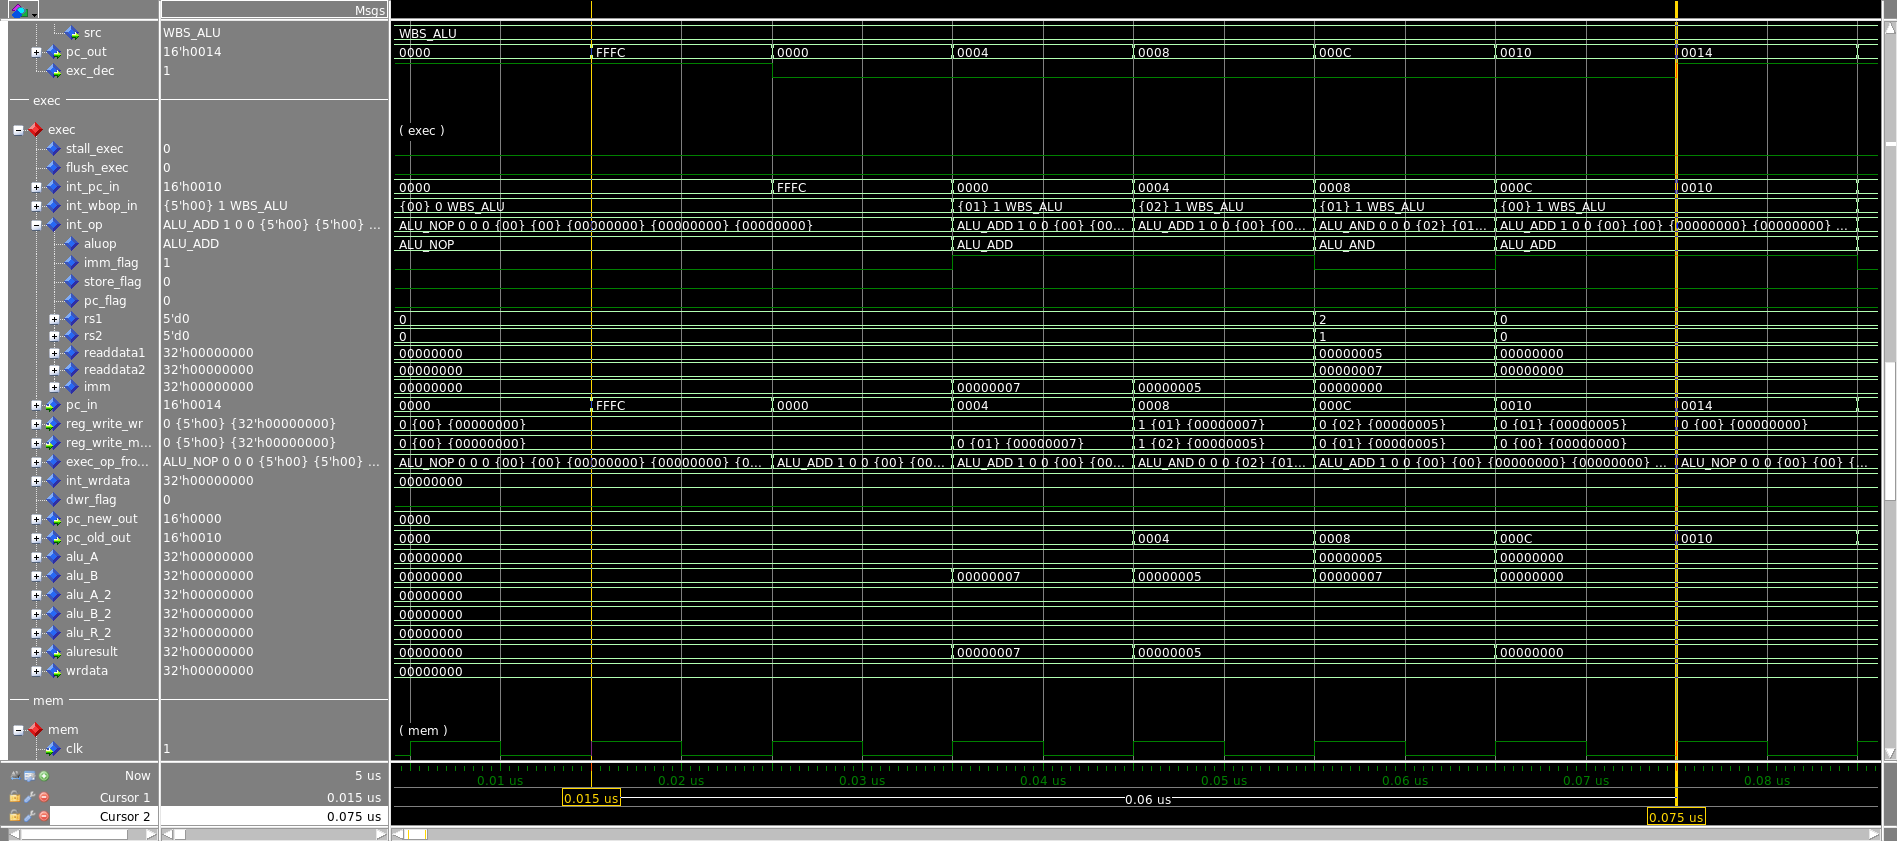
\includegraphics[width=1.0\linewidth]{task_1_exec.png}
\caption{What's going on in the exec stage.}
\label{fig:sim3}
\end{figure}

A screenshot of the exec stage is also appended. 
\newline


Make sure that at least the following signals are visible in
Figure~\ref{fig:sim1}: the program counter in the fetch stage, the
instruction being fetched, the content of registers \texttt{x1} 
and \texttt{x2} as well as the signals \texttt{wraddr},
\texttt{wrdata} and \texttt{regwrite} of the register file.

\begin{lstlisting}[language=,mathescape=false,float=ht,caption={Assembler example with forwarding},label=lst:asmfwd_1]
        addi x1, x0, 7
        addi x2, x0, 5
        and x1, x2, x1
        nop
        nop
\end{lstlisting}

